\documentclass[twocolumn]{revtex4}

\usepackage{graphicx,epsfig}
\usepackage{amsmath}
\usepackage{amsfonts}
\usepackage{fancyhdr}
\usepackage{siunitx}


\begin{document}

\pagestyle{fancy}
\lhead{\bf Verifying open clusters using the Gaia catalogue}
\rhead{Daniel Monzonís Laparra}
\lfoot{Treball de Fi de Grau}
\rfoot{Barcelona, January 2018}


\title{Verifying open clusters using the Gaia catalogue}
\author{Author: Daniel Monzonís Laparra}
\affiliation{Facultat de Física, Universitat de Barcelona, Diagonal
645, 08028 Barcelona, Spain.}
\author{Advisor: Tristan Cantat-Gaudin}
%\date{\today}

\begin{abstract}
{\bf Abstract:} The aim of this work is to study several open clusters that have been previously identified, but using the newer and more precise data from the Gaia DR2 catalogue, trying to verify their existence, and determine an approximation of their age and the amount of interstellar extinction.
\end{abstract}

\maketitle

\section{Introduction}
Open clusters are groups of stars formed from the same molecular cloud simultaneously, and therefore the stars in the cluster share many properties like age, position, proper motion and composition. Because of this, many of these properties can be estimated much more easily from a cluster than from a single star. This information can then be used to trace the structure of the Milky Way, and makes open clusters very interesting for studying stellar evolution and stellar structure, since the only parameter that varies is the mass of each star.

Over 1200 open clusters have been identified within the Milky Way, but it is thought that there exist around $10^5$ open clusters in the galaxy, since most open clusters form near the galactic plane, where the interstellar extinction is higher due to the higher amount of dust, making their observation much harder.\cite{star-clusters}

With the new release of data from Gaia, we can study open clusters with more precision than ever before. This data includes positions in the sky, proper motions, parallaxes, and magnitudes in three different photometric filters for over 1 billion stars.

Using the data from the UCAC4 catalogue, Sampedro et al.\cite{sampedro} reported the existence of 1876 open clusters, using three different membership methods. With the release of the Gaia DR2 catalogue, which contains more precise astrometric data, it is now possible to find and verify the existence of clusters more accurately.
There have already been attempts to identify open clusters using the Gaia DR2 catalogue, for instance, in the study of Cantat-Gaudin et al.\cite{cantat-gaudin}, 1269 clusters have been identified with the new data. Our first goal will be to crossmatch the data from both studies to find the clusters that haven't already been verified.

In this work, we will study some open clusters from both articles, focusing on clusters found in Sampedro's article but that have not been yet verified with the data from Gaia. We will also find estimates for the age and interstellar extinction of these clusters.


\section{The Gaia DR2 catalogue}
The second release of data from Gaia, the Gaia DR2 catalogue\cite{gaiadr2}, introduces high-precision measurements of various astrometry parameters, like proper motions and parallaxes, as well as photometric information for a total of $1 692 919 135$ sources. The catalogue contains a 5-parameter astrometric solution for over 1.3 billion stars, which include the position in the sky given by the right ascension and declination, the proper motion and the parallax. For the rest of the stars, which are the very faint ones ($G > 21$), a 2-parameter astrometric solution is given instead, with only the positions in the sky.

For bright stars ($G < 15$) the uncertainty in the positions and parallax is about $0.02-0.04\ \si{mas}$, and the uncertainty in the proper motions is about $0.07\ \si{mas.yr^{-1}}$. We will only be working with stars of at most $G = 17$, for which the uncertainty in the positions and parallax is of $0.1\ \si{mas}$ and of $0.2\ \si{mas.yr^{-1}}$ in the proper motions. Figure \ref{ppmxl_vs_gaiadr2} illustrates how this data is much more precise than what was available before, by comparing the proper motions of a well known cluster with the data from the PPMXL catalogue\cite{ppmxl} and Gaia DR2.

\begin{figure}[h!]
\centering
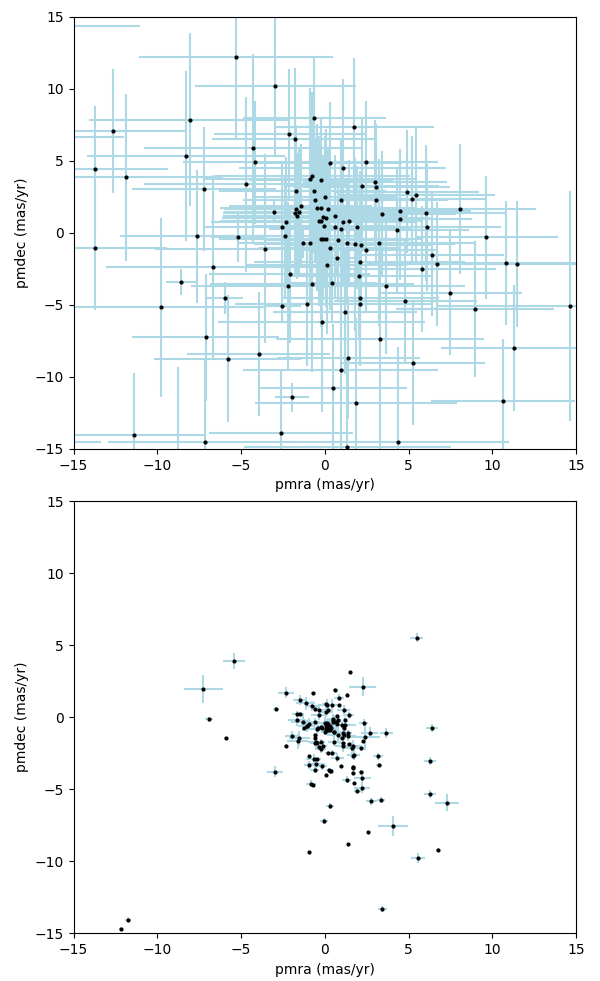
\includegraphics[scale=0.45]{ppmxl_vs_gaia_motions}
\caption{Comparison of the data from PPMXL and Gaia DR2 for the proper motions of the cluster Ivanov 2 \cite{ivanov}.}
\label{ppmxl_vs_gaiadr2}
\end{figure}


The catalogue also lists valuable information on the photometry of most of its sources on the $G$, $G_{BP}$ and $G_{RP}$ photometric passbands. This information will be very useful when determining the age of the clusters we will study, by using a colour-magnitude diagram.


\section{Identifying open clusters}

As a first measure to reduce the number of clusters that need to be verified, we will only check the clusters whose name is not present in the data from both studies. We end up with a list of 890 clusters, due mainly to naming inconsistencies and to the new study possibly missing some clusters found by the old one.

For each of these 890 clusters, we compute the mean right ascension $\alpha$ and declination $\delta$, which we will use as the center point of a circle with radius $\dfrac{\max(D) - \min(D)}{2}$ where $D$ is the set of declinations for all the stars of each cluster. Then, we query the data from the Gaia DR2 catalogue for the region encompassed by this circle. We get stars with a magnitude $G < 17$, since the data from the UCAC4 catalogue does not show stars fainter than $G = 17$. This gives us the data for all the stars in the queried region, so we crossmatch this data with the data from the original study to leave only the stars that are supposedly part of the open cluster. To detect and filter the repeated cases due to name inconsistencies, the center positions of the already verified clusters are also added in the position plots.

\begin{figure*}
\centering
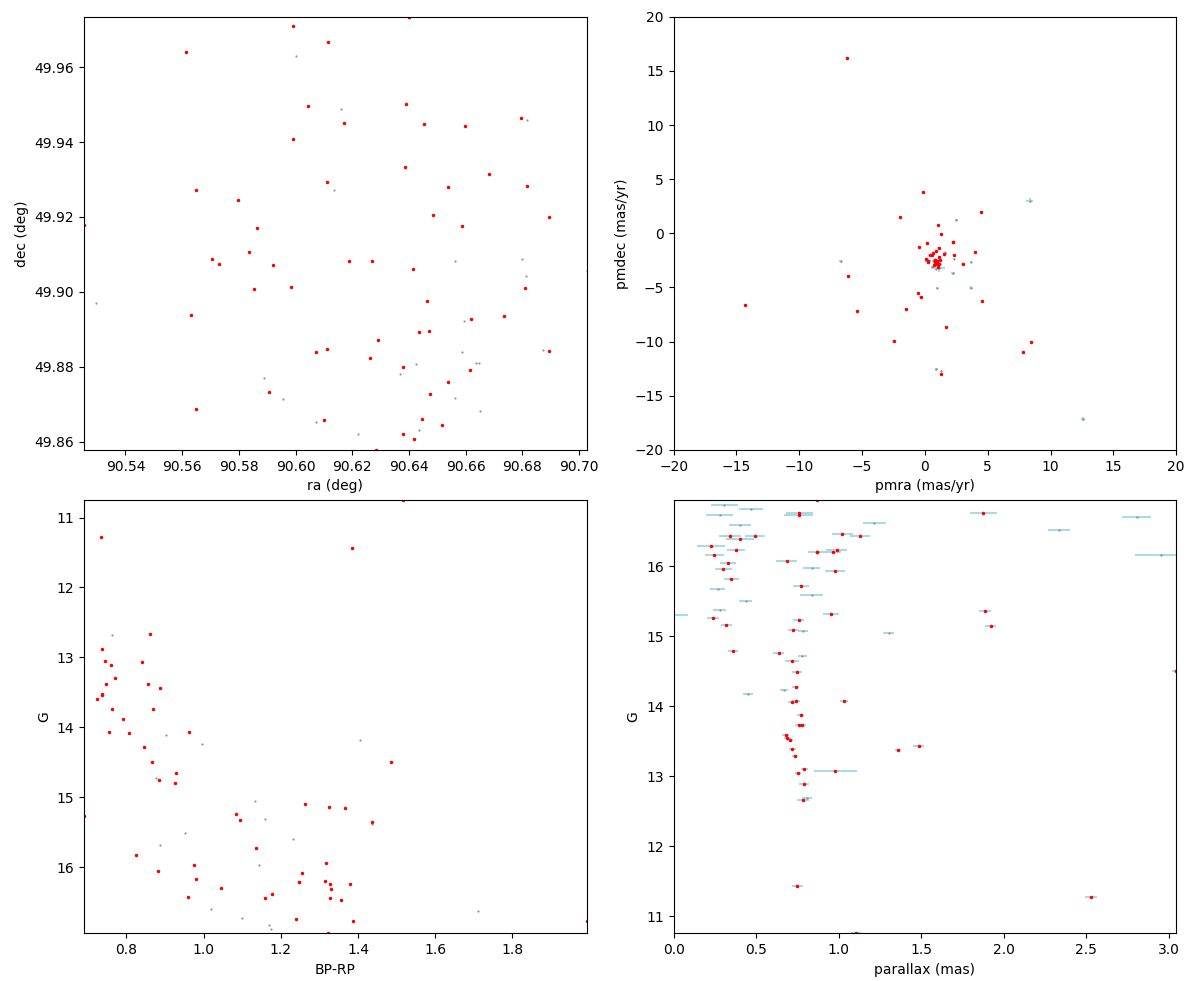
\includegraphics[scale=0.5]{NGC_2126_crossmatch}
\caption{Crossmatched data from the candidate cluster NGC 2126. The red dots correspond to stars from the Gaia DR2 catalogue that match a star from Sampedro's study.}
\label{crossmatched_data}
\end{figure*}

Figure \ref{crossmatched_data} shows one example of the plots that were made for each of the clusters, for one of the cases that are confirmed to be a cluster and that will be studied in the next section to determine its age and interstellar extinction. Note that, in this case, the proper motion space is pretty compact, and there is a clear straight line in the parallax versus magnitude plot, showing that the stars are moving together and are at the same distance. In the color-magnitude diagram, we can see that some stars have already left the main sequence. We will study this in more detail in the following section.


\section{Determining the age and interstellar extinction of the cluster}
In this section we discuss the procedure followed to determine an approximation of the age and interstellar extinction of some clusters. We try this method for a total of 14 clusters, some of which are taken from the list of verified clusters in the study of Cantat-Gaudin, and the rest are cases from the study of Sampedro which we have verified in the previous section. The complete list of tested clusters, as well as some data on them, can be found in Table \ref{tab:clusters}. %TODO comment on the method used to get the members of the cluster
Note that a lower parallax means a greater distance.

\begin{table}[h!]
\begin{tabular}{|l|c|c|c|}
\hline
\textbf{Cluster} & \textbf{Position (deg)} & \textbf{Parallax (mas)} & \textbf{Members} \\
\hline
Alessi 3 & $(109.95, -46.05)$ & $3.5619$ & $243$ \\
\hline
Berkeley 100 & $(351.48, 63.78)$ & $0.1461$ & $57$ \\
\hline
Collinder 421 & $(305.83, 41.69)$ & $0.8169$ & $283$ \\
\hline
ESO 332 08 & $(253.80, -40.96)$ & $0.5332$ & $417$ \\
\hline
Herschel 1 & $(116.72, 0.15)$ & $3.3385$ & $149$ \\
\hline
NGC 752 & $(29.24, 37.77)$ & $2.2245$ & $263$ \\
\hline
NGC 1039 & $(40.51, 42.74)$ & $1.9350$ & $659$ \\
\hline
NGC 2126 & $(90.65, 49.91)$ & $0.7490$ & $151$ \\
\hline
NGC 2169 & $(92.12, 13.94)$ & $0.9863$ & $133$ \\
\hline
NGC 2287 & $(101.51, -20.70)$ & $1.3503$ & $673$ \\
\hline
NGC 2360 & $(109.44, -15.63)$ & $0.8994$ & $695$ \\
\hline
NGC 2479 & $(118.76, -17.73)$ & $0.6311$ & $159$ \\
\hline
Ruprecth 8 & $(105.41, -13.56)$ & $0.4278$ & $138$ \\
\hline
Stock 6 & $(35.93, 63.79)$ & $0.9536$ & $144$ \\
\hline
\end{tabular}
\caption{List of clusters that have been studied, and their mean position (given in ($\alpha$, $\delta$)) and mean parallax, computed using the data from Gaia DR2, and the number of member stars of the cluster.} %TODO mention method name
\label{tab:clusters}
\end{table}

To determine the age and interstellar extinction of the clusters, we make use of the stellar evolution model. Stars enter the main sequence soon after their birth, where they stay most of their life burning hydrogen. When their hydrogen cores deplete, they leave the main sequence and start burning the helium in their core resulting from the fusion of hydrogen atoms. When this happens, the stars maintain a similar brightness, but become much redder in color. The brighter a star is, the faster it will burn through its hydrogen core and leave the main sequence.

If we represent the stars in an open cluster in a Hertzsprung–Russell diagram (HRD), one can see the brightness at which the stars are starting to leave the main sequence. This is called the turnoff point, and it can be used to estimate the age of the cluster.

To be able to represent the data from Gaia in a HRD, we need to use the distance modulus to shift from apparent to absolute magnitude, and we also need to take into account the interstellar extinction, which makes the stars appear redder and less bright than what they actually are.

%%%%%%%%%% Maybe do distance modulus derivation in an appendix?
Let $M$ be the absolute magnitude, and $m$ the apparent magnitude without any corrections due to the interstellar reddening. Then, the distance modulus is just $\mu = m - M$. Since we don't have the absolute magnitude, we need to relate this to the distance of the stars in the cluster, which is given by the parallax.

Remember that
\[m = -2.5 \log_{10} \left( \frac{F(d)}{F_0} \right) \]
where $F$ is the observed flux density of the star, and $F_0$ is the reference flux. %TODO complete this
The absolute magnitude $M$ is the apparent magnitude of the star if it was placed at a distance of $10$ parsecs. The flux $F$ and luminosity $L$ of a star are related by the distance to the star $d$ by
\[F = \frac{L}{4 \pi d^2}\]
and since the luminosity is an intrinsic property of a star, we find the relation
\begin{equation}
\frac{F_1}{F_2} = \left( \frac{d_2}{d_1} \right)^2
\end{equation}
Then, using this relation in the expression $m - M = -2.5 \log_{10} \left( \frac{F(d)}{F(d=10)} \right)$, one can rewrite the distance modulus in terms of the distance as
\begin{equation}
\label{distance-modulus}
\mu = m - M = 5 \log_{10} \left( \frac{d}{10} \right)
\end{equation}
where $d$ is in parsecs. We can use equation \ref{distance-modulus} with the data from Gaia, since the relation between the parallax $p$ given in arcseconds and the distance $d$ given in parsecs is just $d = p^{-1}$.

Given that the stars in an open cluster are relatively close together, we shift every star in the plot by the distance modulus of the mean parallax of the cluster. Now that we are working in the absolute magnitude space, with the exception of the reddening due to the interstellar extinction , we can begin the process of isochrone fitting.

An isochrone is the line that would be drawn in a HRD if we varied the mass of the star at a fixed age. Since the stars in an open cluster have the same age, we can find an isochrone that fits the HRD of the stars in the cluster to determine its age.
The isochrones used are from the PARSEC\cite{parsec}, with the photometric system from Gaia DR2\cite{gaiadr2}, and including the interstellar extinction $A_V$ on a star-to-star basis\cite{girardi}. The metallicity value used for the isochrones is $Z = 0.0152$.  An example of the result of fitting an isochrone to the cluster data can be seen in Figure \ref{nice-isochrone}.

\begin{figure}[h!]
\centering
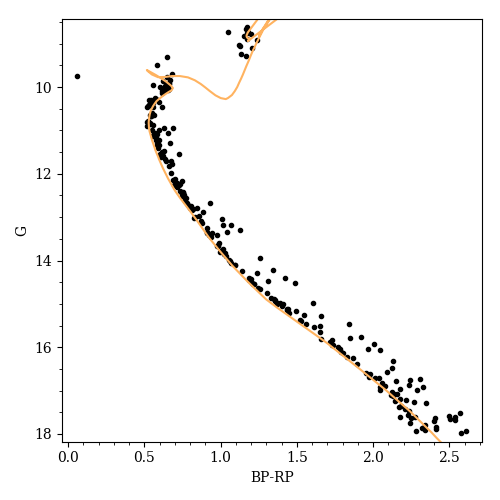
\includegraphics[scale=0.65]{NGC_752}
\caption{HRD of the cluster NGC 752, with an isochrone of age $1.78 \si{Gyr}$ and $A_V = 0.1$, with a shift in total magnitude given by the mean distance modulus $\bar{\mu} = 8.264$.}
\label{nice-isochrone}
\end{figure}

The estimated ages and interstellar extinction $A_V$ for all the clusters studied is shown in Table \ref{tab:fitting-results}.

\begin{table}[h!]
\begin{tabular}{|l|c|c|}
\hline
\textbf{Cluster} & \textbf{Age ($\si{Gyr}$)} & \textbf{$A_V$} \\
\hline
Alessi 3 & $[0.79, 1.00]$ & $[0.0, 0.1]$ \\
\hline
Berkeley 100 & $[0.25, 0.71]$ & $[3.0, 3.4]$ \\
\hline
Collinder 421 & $[0.10, 0.20]$ & $[2.0, 2.3]$ \\
\hline
ESO 332 08 & $[0.32, 0.50]$ & $[2.0, 2.2]$ \\
\hline
Herschel 1 & $[0.32, 0.50]$ & $[0.0, 0.1]$  \\
\hline
NGC 752 & $[1.41, 1.78]$ & $[0.1, 0.2]$  \\
\hline
NGC 1039 & $[0.08, 0.13]$ & $[0.4, 0.5]$  \\
\hline
NGC 2126 & $[0.50, 1.12]$ & $[0.7, 0.9]$ \\
\hline
NGC 2169 & $[0.01, 0.02]$ & $[0.6, 0.7]$ \\
\hline
NGC 2287 & $[0.16, 0.25]$ & $[0.1, 0.2]$ \\
\hline
NGC 2360 & $[0.89, 1.12]$ & $[0.3, 0.4]$ \\
\hline
NGC 2479 & $[1.00, 1.26]$ & $[0.2, 0.3]$ \\
\hline
Ruprecth 8 & $[0.45, 0.79]$ & $[1.0, 1.2]$ \\
\hline
Stock 6 & $[0.45, 0.63]$ & $[1.5, 1.6]$ \\
\hline
\end{tabular}
\caption{Estimated ages and interstellar extinction $A_V$ for the clusters studied via isochrone fitting, given in ranges.}
\label{tab:fitting-results}
\end{table}

\section{Problems when fitting isochrones}
\subsection{Blue stragglers}
Talk about blue stragglers, show some plots where they clearly appear...

\subsection{Binary sequences}
Talk about binary sequences due to binary stars.

\subsection{Differential extinction}
Talk about how extinction can change a lot even within the same cluster. Show an example where this happens, where more distant stars have more extinction (we saw one example with Tristan).

\section{Conclusions}


\section{Appendix}


\vspace*{0.5cm}
\begin{acknowledgments}

\end{acknowledgments}


\begin{thebibliography}{99}

\bibitem{sampedro} L. Sampedro, W. S. Dias, E. J. Alfaro, H. Monteiro, and A. Molino, (2017), arXiv:1706.05581 [astro-ph.SR].

\bibitem{cantat-gaudin} T. Cantat-Gaudin, C. Jordi, A. Vallenari, et al., (2018), arXiv:1805.08726 [astro-ph.GA]

\bibitem{star-clusters} K. Janes, \textsl{Star Clusters}, Encyclopedia of Astronomy and Astrophysics, (Nature Publishing Group, 2001)

\bibitem{gaiadr2} A.G.A. Brown, A. Vallenari, T. Prusti et al., (2018), arXiv:1804.09365 [astro-ph.GA]

\bibitem{ppmxl} S. Roeser, M. Demleitner and E. Schilbach, (2010), arXiv:1003.5852 [astro-ph.GA]

\bibitem{ivanov} A. L. Tadross, R. Bendary, (2014), arXiv:1403.3014 [astro-ph.GA]

\bibitem{parsec} A. Bressan, P. Marigo, L. Girardi, B. Salasnich, C. Dal Cero, S. Rubele, and A. Nanni, (2012), arXiv:1208.4498 [astro-ph.SR]

\bibitem{girardi} L. Girardi, J. Dalcanton, B. Williams, et al., (2008), arXiv:0804.0498 [astro-ph]


\end{thebibliography}


\end{document}
